\subsection{D-Wave Hybrid BQM with an explicit ten-second limit}
\label{sec:dwavehybrid}
We submitted the same three frozen models to the real Leap Hybrid BQM service, under default,
penalty TPE and single-agent policies. This service is distinct from direct QPU sampling.
The experiment completed 27 of 27 conditions and used 72 solver submissions.
Each condition allowed at most three calls. Every call explicitly set the service time limit
to ten seconds; a model requiring a larger minimum was refused before submission rather than
given a longer limit. Sequential execution was bounded by 81 calls and 810 service seconds.
A read-only retrieval of 72 completed answers reported total service charge time
of 719.495 seconds. The original ledger conservatively reserved ten seconds per call;
the answers also report 42.526 seconds of aggregate internal QPU access,
positive for 72 of 72 answers. These are hybrid-service timings, not direct-QPU runs.
measured service timings are preserved separately. Network and inference time are additional.
\begin{table}[t]\centering\small
\caption{Real Hybrid BQM comparison. Gaps use exact references for the three frozen models; wall time includes network and inference.}
\begin{tabular}{@{}llrrrr@{}}\toprule Model & Policy & Feasible & Gap & Calls & Wall s \\\midrule
wine & default & 3/3 & 0.0000 & 3.00 & 43.4 \\
wine & penalty\_tpe & 3/3 & 0.0000 & 3.00 & 43.6 \\
wine & agent & 3/3 & 0.0000 & 1.00 & 52.3 \\
knapsack60 & default & 3/3 & 0.1060 & 3.00 & 42.0 \\
knapsack60 & penalty\_tpe & 3/3 & 0.1164 & 3.00 & 41.9 \\
knapsack60 & agent & 3/3 & 0.1149 & 3.00 & 123.5 \\
select80 & default & 3/3 & 0.0000 & 3.00 & 44.8 \\
select80 & penalty\_tpe & 3/3 & 0.0141 & 3.00 & 43.6 \\
select80 & agent & 3/3 & 0.0016 & 2.00 & 97.2 \\
\bottomrule\end{tabular}\end{table}
\begin{figure}[t]\centering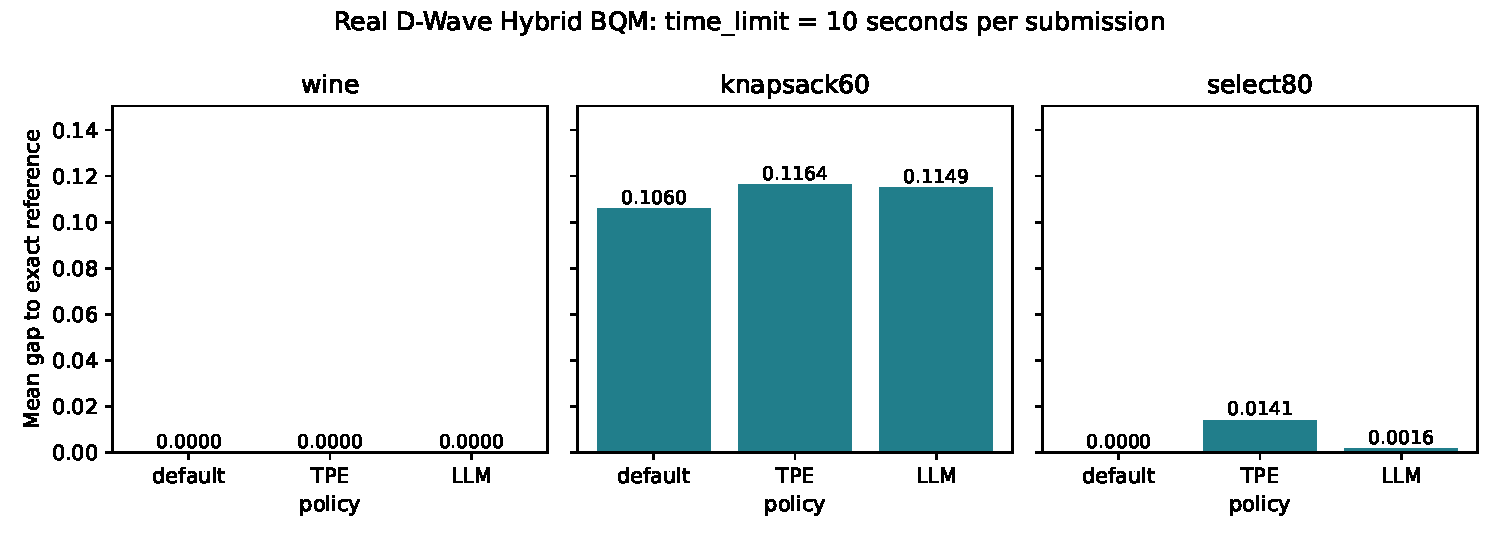
\includegraphics[width=\linewidth]{figures/dwave_hybrid_comparison.pdf}
\caption{Real hybrid-service results with an explicit ten-second limit.}\end{figure}
The three repetitions are external resubmissions, without exposed hardware RNG seeds.
The ten-second Hybrid ceiling and earlier three-second CGA ceiling are different resource
allocations. They do not establish a hardware advantage, nor a held-out knowledge-transfer result.
